%  Typ dokumentu - článek, prezentace aj.
\documentclass[english]{article}

%  Nastaví vstupní a výstupní kódování znaků (encoding) a lokalizace
\usepackage[T1]{fontenc}
\usepackage[utf8]{inputenc}
\usepackage[english,czech]{babel}
\usepackage{icomma}

%  Formát papíru a odsazení od jeho okrajů
\usepackage[letterpaper]{geometry}
\geometry{verbose,tmargin=1.5cm,bmargin=2cm,lmargin=2cm,rmargin=2cm}

%  Umožňuje pracovat s grafikou
\usepackage{graphicx}
\usepackage{bigstrut}
\usepackage{epstopdf}

%  Automaticky odsadí i první paragraf v každé sekci
\usepackage{indentfirst}

%  Umožňuje rozdělovat obsah na více sloupců
\usepackage{multicol}
\usepackage{booktabs}
\usepackage{pgffor}

% physics
\newcommand{\unit}[1]{\ \mathrm{#1}}
\newcommand{\dd}{\mathrm{d}}
\newcommand{\ee}{\mathrm{e}}

%  Umožňuje používat hypertextové odkazy, nastavuje jejich barvu a
%  vlastnosti
\usepackage[unicode]{hyperref}
\hypersetup{
colorlinks=true, citecolor=blue, filecolor=blue, linkcolor=blue,
urlcolor=blue
}

%  Formátování stránek, empty = odstraní číslování
% \pagestyle{empty}

%  Řádkování
\linespread{1.2}

%  Lepší zobrazování matematiky (rozšíření sum o \limits atd.)
\everymath{\displaystyle}
\usepackage{amsmath, amsthm, amssymb}

% Umožní psát přes \mathbb{N/R/Q/..} množiny čísel
\usepackage{amssymb}

%  Velikost fontu matematických výrazů v dokumentu lze pro danou
% základního fontu dokumentu upravit pomocí:
% \DeclareMathSizes{X}{Y}{Z}{U} kde:
% X je velikost fontu v dokumentu, pro kterou se matematika upraví
% Y je standartní velikost fontu matematiky
% Z je velikost fontu zmenšených (vnořených výrazů)
% U je velikost fontu ještě více zmenšených (vnořených výrazů).
\DeclareMathSizes{10}{10.5}{9}{9}

%  Nastaví autora, název, datum, skupinu měření apod. (můj vlastní
% příkaz, umožní znovu-použití v dokumentu)
\newcommand{\Author}{David Roesel}
\newcommand{\Coauthor}{Tereza Schönfeldová}
\newcommand{\Institute}{FJFI ČVUT v Praze}
\newcommand{\Subject}{FYZIKÁLNÍ PRAKTIKUM II}
\newcommand{\Group}{7}
\newcommand{\Circle}{ZS 7}
\newcommand{\Title}{Úloha \#1  \\Kondenzátor, mapování elektrostatického pole}
\newcommand{\Date}{7.4.2014}

% Začátek dokumentu - Formátování na výstup
\begin{document}

% Interní proměnné, možno zobrazovat u prezentací, používají se při
% generování pomocí \titlepage apod.
\author{\Author}
\title{\Title}
\date{\Date}

%  Lokalizace některých názvů do češtiny
\renewcommand{\figurename}{Obr.}
\renewcommand{\tablename}{Tab.}
\renewcommand{\refname}{Reference}

% --- Hlavička dokumentu -----------------------------------------------

\setlength{\parindent}{0cm}
\begin{multicols}{2}
\textbf{\Subject \\
        \Institute \\[0.1cm]
%\large  \Title \\[0.5cm]
\Title \\[0.5cm]
}
\begin{tabular}{rlrl}
\large Datum měření: & \Date & \large Skupina: & \Group \\
\large Jméno: & \Author & \large Kroužek:  & \Circle\\
\large Spolupracovala: & \Coauthor &\large Klasifikace:\\
\end{tabular}

\begin{flushright}

\includegraphics[scale=0.28]{../../_meta/fjfi_standart.pdf}
\hspace{0.2cm}
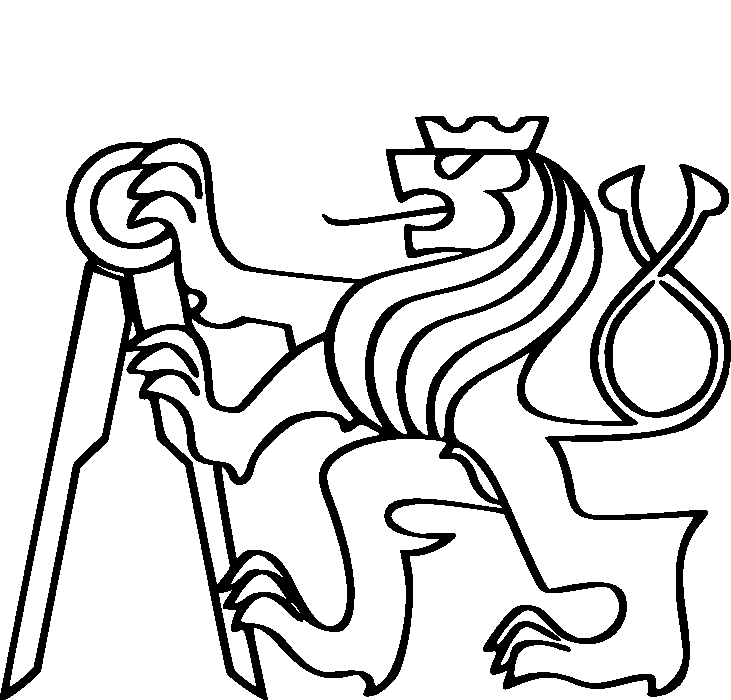
\includegraphics[scale=0.28]{../../_meta/cvut_standart.pdf}
\end{flushright}
\end{multicols}
\hrule
\vspace{0.5cm}

% ----------------------------------------------------------------------


% --- Tělo dokumentu ---------------------------------------------------
\setlength{\parindent}{0.5cm}
\section{Pracovní úkoly}
\begin{enumerate}
\item DÚ: Odvoďte kapacitu deskového kondenzátoru.
\item DÚ (Deskový kondenzátor): Bezpečnostní normy obvykle připouštějí maximální náboj $Q_{max}$ na deskách kondenzátoru, kterému odpovídá určité napětí $U_{max}$ mezi těmito deskami. Stanovte závislost poměru plochy desek kondenzátoru $S$ a vzdálenosti mezi nimi $d$ ${S}/{d}$ v případě deskového kondenzátoru jako funkci náboje $Q_{max}$ a napětí $U_{max}$. Následně spočítejte hodnotu poměru ${S}/{d}$ pro vzduchový deskový kondenzátor, kde $Q_{max} = 50~\mathrm{\mu C}$
a $U_{max} = 100~\mathrm{kV}$. 

\item Změřte průrazné napětí $U$ mezi deskami kondenzátoru pro deset různých vzdáleností desek $d$. Náboj tedy přivádějte až do průrazu mezi deskami kondenzátoru. Průrazné napětí $U$ určete prostřednictvím silového působení na
vahách ve chvíli průrazu a vztahu (12) z \cite{bib:zadani}. Z naměřených hodnot průrazného napětí $U$ pro různé vzdálenosti $d$ určete
následně dielektrickou pevnost vzduchu a porovnejte s tabulkovou hodnotou pro suchý vzduch. Diskutujte důvod případné odlišnosti hodnot.

[BONUS]: Nalezněte empirický vztah, který popisuje chování hodnoty dielektrické pevnosti vzduchu vůči podmínkám v místnosti (tlak, teplota, vlhkost, atd.) a určete hodnotu dielektrické pevnosti vzduchu pro tyto parametry.

\item Změřte přitažlivé síly mezi deskami kondenzátoru pro tři různé vzdálenosti desek $d$. Náboj přivádějte až do průrazu na kulovém jiskřišti s mikrometrickým šroubem paralelně připojenému k deskovému kondenzátoru. Volte deset různých hodnot doskoku $s$ pro každou vzdálenost mezi deskami kondenzátoru $d$. Ze silového působení spočítejte napětí podle (12) v \cite{bib:zadani} a ze vztahu (13) v \cite{bib:zadani} určete hodnoty neznámé funkce $f(s/D)$ pro konkrétní poměr $s/D$. Všech třicet určených hodnot $f(s/D)$ vyneste do společného grafu závislosti $f(s/D)$ na poměru $s/D$. Vzhledem k podmínce (14) v \cite{bib:zadani} a monotónnosti funkce u doskoku $s$ zvolte vhodný tvar funkce $f(s/D)$ popisující chování naměřených dat, kterým všech třicet bodů grafu nafitujte. Jako výsledek uveďte hodnoty a chyby fitovacích parametrů zvolené funkce $f(s/D)$.

[BONUS]: Bonusové body lze získat za volbu tvaru funkce $f(s/D)$, který bude vhodně popisovat chování grafu.

\item Zvolte si dvě konfigurace elektrod, nastavte na nich napětí cca 10~V a zmapujte potenciál v síti $12\times12$ bodů. Data si vyzálohujte a v domácím vyhodnocení proveďte důkladné zpracování. 

[BONUS]: Zmapujte třetí konfiguraci elektrod.

\end{enumerate}

	
\section{Vypracování}

	\subsection{Použité přístroje}
		Wimshurstova elektrika, váhy, deskový kondenzátor, podstavec, vodiče, kulové jiskřiště, zkratovač, PC, regulovatelný zdroj 12~V, souprava pro mapování elektrostatického pole, programy \emph{GNUplot} a \emph{Python}.
			
	\subsection{Teoretický úvod}
		\subsubsection{Energie elektrostatického pole, síla mezi deskami kondenzátoru}
		Na spočítání energie kondenzátoru se dá využít práce potřebné pro jeho nabití. Budeme uvažovat kondenzátor s kapacitou $C$ a s elektrodami nabitými na náboje $+q$ a $-q$. Budeme-li chtít přenést elementární náboj z jedné desky na druhou přes potenciálový rozdíl $U = q/C$, budeme muset vykonat práci rovnou
		\begin{equation}
		W = \int_{0}^{Q}U \dd q = \int_{0}^{Q} \frac{q}{C} \dd q = \frac{Q^2}{2C} = \frac{C U^2}{2}.
		\end{equation}
		
		Z odvození uvedeného níže plyne pro deskový kondenzátor vztah 
		\begin{equation}
		C = \frac{\varepsilon_0 \varepsilon_r S}{d},
		\end{equation}
		kde $\varepsilon_0$ je permitivita vakua, $\varepsilon_r$ relativní permitivita prostředí (mezi deskami) a $d$ vzdálenost obou desek (každé  o ploše $S$). Vezmeme-li v potaz, že uvažujeme pouze vzduchový kondenzátor a měříme s dostatečně velkými chybami, můžeme si dovolit aproximovat $\varepsilon_r \approx 1$ a ze vzorců ho tak vyřadit.
		
		Z předchozích vztahů se spolu s rovností $U = E\cdot d$ dá získat pro práci
		\begin{equation}
		W = \frac{\varepsilon_0 E^2 V}{2} = w_E V,
		\end{equation}
		kde $V = S\cdot d$ je objem, který uzavírají desky kondenzátoru, a $w_E = \frac{1}{2} \varepsilon_0 E^2$ je objemová hustota energie elektrického pole.
		
		Sílu, kterou se navzájem přitahují desky kondenzátoru, můžeme odvodit ze změny energie při infinitezimálním posunutí desek kondenzátoru. Získáme tedy
		\begin{equation}\label{eq:SilaMeziDeskamiKondenzátoru}
		F = \frac{\dd W}{\dd d} = \frac{\dd }{\dd d} \frac{1}{2} \varepsilon_0 E^2 S d = \frac{\varepsilon_0 E^2 S}{2} = \frac{\varepsilon_0 U^2 S}{2 d^2}.
		\end{equation}
		
		\subsubsection{D.Ú.: Kapacita deskového kondenzátoru -- odvození}
		Máme-li kondenzátor nabitý s konstantní plošnou hustotou $\sigma$, bude mezi jeho deskami homogenní elektrické pole o intenzitě
		\begin{equation} \label{eq:C_odovoz_1}
		E = \frac{\sigma}{\varepsilon}.
		\end{equation}
		
		Mezi nábojem na kondenzátoru $Q$, jeho kapacitou $C$ a napětím mezi deskami $U$ platí vztah
		\begin{equation} \label{eq:C_odovoz_2}
		U = \frac{Q}{C}
		\end{equation}
		a zároveň platí pro napětí a intenzitu elektrického pole 
		\begin{equation} \label{eq:C_odovoz_3}
		U = Ed,
		\end{equation}
		kde $d$ je vzdálenost desek kondenzátoru. Pokud do vztahu (\ref{eq:C_odovoz_3}) dosadíme za $U$ ze vztahu (\ref{eq:C_odovoz_2}), dostáváme
		\begin{equation} \label{eq:C_odovoz_4}
		C = \frac{Q}{Ed}.
		\end{equation}
		Dále můžeme ze vztahu (\ref{eq:C_odovoz_1}) dosadit za $E$, abychom dostali 
		\begin{equation} \label{eq:C_odovoz_5}
		C = \frac{\varepsilon Q}{d \sigma}.
		\end{equation}
		
		Plošná hustota elektrického náboje $\sigma$ je definovaná jako 
		\begin{equation} \label{eq:C_odovoz_6}
		\sigma = \frac{Q}{S},
		\end{equation}
		kde $Q$ je náboj rozložený na ploše $S$.
		
		Dále stačí z posledního vzorce dosadit za $\sigma$ do (\ref{eq:C_odovoz_5}) a dostáváme výsledný vztah pro kapacitu deskového kondenzátoru 
		\begin{equation} \label{eq:C_odovoz_7}
		C = \frac{\varepsilon S}{d}.
		\end{equation}
		
		\subsubsection{Dielektrická pevnost vzduchu}
		Dielektrická pevnost vzduchu $E_p$ nám říká, jaká musí být intenzita elektrického pole, aby se vzduch stal vodivým a došlo k průrazu. $E_p$ se tedy podle (\ref{eq:C_odovoz_3}) bude rovnat
		\begin{equation}
				E_p=\frac{U_p}{d},
				\label{eq:Ep}
		\end{equation}
		kde $U_p$ je napětí potřebné k průrazu a $d$ je tloušťka vrstvy vzduchu.
		
		\subsubsection{Kulové jiskřiště}
		K měření vysokých napětí se dá využít kulového jiskřiště, které je jedním z nejjednodušších přístrojů pro tento účel. Má-li jasně geometricky definované elektrody a jde-li pro ně matematicky určit tvar pole, dává nám absolutní měřící metodu napětí. Pro kulové jiskřiště ve vzduchu, tvořené dvěma stejně velkými koulemi, bude platit
		\begin{equation} \label{eq:jiskriste}
		U = 27,75 \left( 1 + \frac{0,757}{\sqrt{\delta D}} \right) \frac{\delta s}{f\left(\frac{s}{D}\right)}, \qquad \delta = \frac{b}{760}\frac{273 + 20}{273 + T},
		\end{equation}
		kde $U$ je průrazné napětí [kV], $s$ doskok [cm] (vzdálenost mezi kuličkami jiskřiště), $D$ průměr koulí [cm] a $\delta$ relativní hustota vzduchu. V její definici je pak $b$ barometrický tlak [torr] a $T$ teplota [$^\circ$C]. Funkce $f = f(s/D)$ je závislá na poměru $s/D$ a na geometrické pravidelnosti pole. Pro $s/D = 0$ je $f = 1$ a se zvětšujícím se $s$ funkce $f$ roste.
		
		\subsubsection{Mapování elektrostatického pole}
		Elektrické pole $\vec{E}$ můžeme v bodě prostoru definovat jako sílu $\vec{F}$ na jednotkový náboj $q$, tedy podle vztahu
		\begin{equation}
		\vec{E} = \frac{\vec{F}}{q}.
		\end{equation}
		
		Experimentálně se ale mapují lépe ekvipotenciální plochy než samotné napětí. Potenciálový rozdíl $\Delta U$ je definován jako
		\begin{equation}
		\Delta U = \frac{W}{q}.
		\end{equation}
		
		Elektrické pole je potom záporně vzatý gradient potenciálu
		\begin{equation}
		\vec{E} = - \text{grad}\ U.
		\end{equation}
		
		
	\subsection{Postup měření}
						
		\subsubsection{Přitažlivá síla desek kondenzátoru}
				Kovové desky tvořící vzduchový kondenzátor byly připraveny na místě. Vrchní z nich byla zavěšena na provázku, který byl upevněn na vahách, spodní pak nevodivě připevněna ke stojanu se šroubem, který umožňoval regulovat její výšku. K deskám jsme připojili Wimshurstovu elektriku a umístili na vrchní malé závažíčko tak, aby byly desky rovnoběžné. Stojanem se šroubem jsme nastavovali různé vzdálenosti desek, které jsme následně měřili posuvným měřítkem. 
				
				Otáčením kliky na Wimshurstově elektrice jsme na deskách kondenzátoru generovali vysoké napětí a u toho jsme sledovali na vahách aktuální hodnotu hmotnosti. V momentu, kdy nastal průraz vzduchu elektrickým proudem (ať už mezi deskami kondenzátoru pro úkol 3 nebo na kulovém jiskřišti pro úkol 4), jsme odečetli a zaznamenali hodnotu, kterou ukazovaly váhy. Náboj jsme se snažili generovat takovou rychlostí, aby z vah ještě šla odečíst hodnota v momentu průrazu, tedy ze začátku rychle a pomaleji blíže očekávané hodnotě. Při celém experimentu jsme dávali pozor na problémy se zapojením, které mohly nastávat důsledkem přiblížení přívodních kabelů buď navzájem k sobě, nebo k elektrodě s opačnou polaritou. 
				Poté, co proběhl každý z průrazů, jsme vybili kondenzátor a Wimshurstovu elektriku (stačí teoreticky zkratovat jen jedno), aby v obvodu nezůstal zbytkový náboj.
				
				U čtvrtého úkolu jsme dbali toho, aby k průrazu docházelo opravdu na kulovém jiskřišti a ne na kondenzátoru jako v úloze číslo 3. Vzdálenost koulí kulového jiskřiště bylo právě z tohoto důvodu třeba volit vhodným způsobem (zmenšit). Pro každou ze tří vzdáleností desek jsme změřili závislost síly (hmotnosti na vahách) na doskoku (vzdálenosti koulí jiskřiště).
		
		\subsection{Mapování elektrostatického pole}
				V tomto experimentu bylo třeba souřadnicovou síť (A--L)$\times$(1--12) umístit pod skleněnou misku s vodou. Do vody jsme následně umístili elektrody napojené na zdroj napětí 12~V v odpovídající konfiguraci a měřili digitálním voltmetrem napěťový rozdíl mezi jednou z elektrod a daným bodem souřadnicové sítě. Zároveň jsme se snažili měřit opatrně, nepohnout s elektrodami či souřadnicovou sítí a udržovat hrot vodiče voltmetru kolmý ke dnu nádobky. Jako první konfiguraci elektrod jsme zvolili dvě podélné a na sebe rovnoběžné (konfigurace "kondenzátor" - Obr.~5 z \cite{bib:zadani}) o vzájemné vzdálenosti 2~cm. Ve druhé konfiguraci jsme nahradili jednu z podélných elektrod bodovou a nechali ji ve stejné vzdálenosti od té původní a přibližně na jejím středu. Jako třetí bonusovou konfiguraci jsme bodovou elektrodu umístili do středu souřadnicové sítě a podélnou jsme nahradili elektrodou kruhovou (po obvodu nádobky). Ve všech případech byly elektrody opačně polarizovány. 

		\subsection{Naměřené hodnoty}
				\subsubsection{Přitažlivá síla desek kondenzátoru}
						Naměřené hodnoty jsou vyneseny v Tab.~\ref{tab:kondenzator}. Z hmotnosti změřené vahami jsme přenásobením tíhovou konstantou $g=9,81~\unit{ms^{-2}}$ určili přitažlivou sílu mezi deskami kondenzátoru. Permitivitu prostředí jsme uvažovali $\varepsilon_0=8,86\cdot 10^{-12}~\unit{Fm^{-1}}$ a z průměru desek kondenzátoru určeného svinovacím metrem jako $2r=(17,0\pm 0,1)~\unit{cm}$ jsme dopočítali obsah jedné z nich na $S=(227\pm 3)~\unit{cm^2}$. Z těchto hodnot jsme podle (\ref{eq:SilaMeziDeskamiKondenzátoru}) dopočítali průrazné napětí $U$, které jsme využili k výpočtu dielektrické pevnosti vzduchu $E_p$ podle (\ref{eq:Ep}) pro jednotlivá měření. Aritmetickým průměrem (\ref{eq:aritmeticky_prumer}) naměřených hodnot jsme pak získali závěrečnou hodnotu i s chybou (\ref{eq:chyba_aritmetickeho_prumeru}) jako
						\begin{equation}
								E_p = (1,35\pm 0,03)~\unit{MV/m}.
						\end{equation}
				
						Pro úkol s kulovým jiskřištěm (určování neznámé funkce $f(s/D)$) jsou naměřené hodnoty uvedeny v Tab.~\ref{tab:jiskriste}. Ze silového působení jsme, stejně jako v případě minulého úkolu, spočítali napětí $U$. Teplotu v místnosti jsme určili z teploměru v praktiku na $T=(24,5\pm0,1)~\unit{^\circ C}$, barometrický tlak jsme vzhledem k nefunkčnímu barometru brali z \cite{bib:tlak} a uvažovali jsme tedy jeho hodnotu $b=762,81~\unit{torr}$. Průměr koulí kulového jiskřiště jsme určili jako $D=(1,44\pm0,01)~\unit{cm}$. S naměřenými hodnotami doskoku $s$ můžeme dopočítat $f(s/D)$ snadno pomocí (\ref{eq:jiskriste}). Hodnoty $f(s/D)$ jsou vyneseny v závislosti na poměru $s/D$ v grafu na Obr. \ref{fig:g_pruraz}. Body jsme proložili lineární závislostí $f(s/D) = a\cdot(s/D)+1$ (která splňuje naše podmínky) a její parametr určili jako
						\begin{equation}
								a = (1,55\pm0,07).
						\end{equation}
						
				\subsubsection{Mapování elektrostatického pole}
						Grafické zpracování naměřených hodnot při mapování elektrostatického pole ve všech třech konfiguracích je vyneseno v grafech na Obr.~\ref{fig:g_konf1}, \ref{fig:g_konf2} a \ref{fig:g_konf3}. Ke každému z nich dále uvádíme jako ilustrační doplněk pohled ze shora na Obr.~\ref{fig:g_konf1_mapa}, \ref{fig:g_konf2_mapa} a \ref{fig:g_konf3_mapa}.

  					
	\subsection{Diskuse}
			\subsubsection{Dielektrická pevnost vzduchu}
					Při měření hmotnosti na vahách bylo těžké určit správně chybu odečítaných hodnot. Vzhledem k tomu, jak rychle se pohybovaly hodnoty v hledáčku, bylo často velice obtížné zpozorovat hodnotu v momentu výboje. V některých případech jsme z tohoto důvodu museli měření dokonce provádět několikrát, než se nám podařilo v momentu výboje vůbec nějakou hodnotu zahlédnout. Jako odhad uvádíme pro první měření chybu $0,5$~g, je ale dost dobře možné, že byla chyba větší. Vzhledem k tomu, jak jsme hodnoty odečítali, mohlo také během celého měření docházet k systematické chybě tím, že jsme brali vždy vyšší či nižší hodnotu. Pro přesnější měření a určení chyb by bylo záhodno změřit při jedné konfiguraci aparatury (tedy jedné vzdálenosti desek kondenzátoru) několik hodnot a zjistit jejich statistickou chybu. Když jsme totiž opakovali měření pro stejnou vzdálenost desek, podařilo se nám odečíst až o $5$~g rozdílné hodnoty. 
			
					Námi stanovená dielektrická pevnost vzduchu $E_p = (1,35\pm 0,03)~\unit{MV/m}$ je o něco menší než poloviční oproti tabulkové \cite{bib:tabulky} hodnotě $E_{tab} = 3~\unit{MV/m}$. Tato odchylka nejspíše nebude způsobena výše diskutovanými chybami, vzhledem k tomu, že nám hodnoty $E_p$ vycházely v jednotlivých měřeních konzistentní (ač menší). V případě, že by byla naše metoda nedostatečně přesná, pozorovali bychom mnohem ``rozházenější'' hodnoty. Rozdíl oproti tabulkové hodnotě tedy přisuzujeme buď systematické chybě, která vedla k podhodnocení závěrečné hodnoty, nebo ionizaci vzduchu a jeho vlhkosti (tabulková hodnota je definována pro suchý vzduch).
			
			\subsubsection{Kulové jiskřiště}
		 			Při měření s kulovým jiskřištěm nastávaly při určování hmotnosti stejné problémy jako v předchozí úloze, přesnost však byla (vzhledem k menší rychlosti otáčení stupnice) vyšší. Odhadli jsme ji tím pádem na $0,1$~g, ale opět mohla být reálně vyšší, stejně jako mohly být výsledky zatíženy systematickou chybou. Při volbě funkce $f(s/D)$ jsme zohledňovali, že má funkce s rostoucím poměrem $(s/D)$ stoupat, a že $f(0)=1$. Z tohoto důvodu jsme pro naše hodnoty na Obr.~\ref{fig:g_pruraz} zvolili lineární závislost $f(s/D) = a\cdot(s/D) + 1$. Zdá se, že našim hodnotám by o něco více vyhovovala funkce, jejíž míra stoupání by s rostoucím poměrem $(s/D)$ klesala. Další možností by mohla být například funkce $f(s/D)=a\cdot\unit{ln}(s/D+1)+1$, její průběh však na námi fitovaném intervalu vypadá velmi podobně jako u lineární závislosti. 
		 			
		 			Při tomto měření jsme nevolili ekvidistantní kroky $s$ vzhledem k tomu, že jsme s pevně zvoleným krokem při prvním měření narazili na situaci, kdy nám začaly výboje probíhat na kondenzátoru, místo na jiskřišti. Vrátili jsme se tedy na nižší doskoky a změřili některé další hodnoty mezi již naměřenými. Výsledky by to však nemělo ovlivnit. Na nepřesnosti tohoto i předchozího měření mohlo mít vliv mírné houpání desek kondenzátoru, které jsme mohli způsobit při jeho vybíjení. 
	
			\subsubsection{Mapování elektrostatického pole}
					Při určování napětí v jednotlivých bodech sítě nastávalo několik problémů. V první řadě bylo umisťování hrotu vodiče na danou souřadnici nepřesné vzhledem k tomu, že byla souřadnicová síť umístěna pod vrstvou skla, která pozici bodu zkreslovala. Zcela jistě se nám také nepodařilo v průběhu celého měření udržet elektrody přesně na jednom místě vzhledem k jejich chatrnému upevnění, a hrot vodiče voltmetru nešel v naší konfiguraci vždy umístit zcela kolmo na podložku. Napětí na voltmetru značně kolísalo a jeho hodnota tedy bude mít ve skutečnosti větší chybu než uváděných $0,01$~V. Měření by se dalo zpřesnit průměrováním hodnoty přes delší časový interval, měření však bylo relativně časově náročné a nebylo to tak v našich možnostech. Na orientační zmapování pole však naše výsledky bohatě stačí a měření můžeme považovat za úspěšné. Pro detailnější proměření by stálo za to použít nějaký druh automatizace.
	
\section{Závěr}
		Za domácí úkol jsme v přípravě odvodili kapacitu deskového kondenzátoru. Stanovili jsme také závislost poměru plochy desek a vzdálenosti desek kondenzátoru jako funkci napětí $U_{max}$ a náboje $Q_{max}$. Následně jsme spočítali hodnotu poměru $(s/D)$ pro vzduchový deskový kondenzátor za uvažování hodnot $Q_{max}=50~\unit{\mu C}$ a $U_{max}=100~\unit{kV}$. 
		
		Změřili jsme průrazné napětí $U$ mezi deskami kondenzátoru pro 10 různých vzdáleností desek $d$ a z naměřených hodnot jsme určili dielektrickou pevnost vzduchu na $E_p = (1,35\pm 0,03)~\unit{MV/m}$. Rozdíl této hodnoty oproti tabulkové \cite{bib:tabulky} jsme diskutovali. 
		
		Změřili jsme přitažlivé síly mezi deskami kondenzátoru pro tři různé vzdálenosti desek $d$ s průrazy na kulovém jiskřišti paralelně připojenému k deskovému kondenzátoru. Z naměřených hodnot jsme určili závislost funkce $f(s/D)$ na poměru $(s/D)$ a zvolili jsme podle toho její tvar. Všechny naměřené hodnoty jsme nafitovali a vynesli spolu se zvolenou závislostí do grafu na Obr.~\ref{fig:g_pruraz}. Parametr $a$ závislosti $f(s/D) = a\cdot(s/D)+1$ nám vyšel z fitu i s chybou jako $a = (1,55\pm0,07)$.
		
		Zvolili jsme si tři konfigurace elektrod, nastavili jsme na nich napětí 12~V a zmapovali jsme potenciál v síti $12\times12$ bodů. Data jsme zpracovali a vynesli do grafů pomocí programu \emph{Python} a jeho knihovny \emph{matplotlib}. 

\section {Použitá literatura}
% --- Literatura a reference -------------------------------------------
\begingroup
\renewcommand{\section}[2]{}

\begin{thebibliography}{9}
\bibitem{bib:zadani} Kolektiv KF, \emph{Návod k úloze: Kondenzátor, mapování elektrostatického pole} [Online], [cit. \today] \newline http://praktikum.fjfi.cvut.cz/pluginfile.php/414/mod\_resource/content/5/mapovani\_MS\_v2.pdf

%\bibitem{bib:h3} Petr Chaloupka, \emph{Jak zpracovávat data} [Online], [cit. \today] \newline  https://dl.dropboxusercontent.com/u/11296940/zfm/h3.pdf

%\bibitem{bib:navody} Kolektiv KF, \emph{Návody k přístrojům} [Online], [cit. \today] \newline http://praktikum.fjfi.cvut.cz/documents/chybynav/navody-o.pdf

\bibitem{bib:chyby} Kolektiv KF, \emph{Chyby měření} [Online], [cit. \today] \newline http://praktikum.fjfi.cvut.cz/documents/chybynav/chyby-o.pdf

%\bibitem{bib:ctverce} Kolektiv KACH UPOL, \emph{Hodnocení analytických výsledků} [Online], [cit. \today] \newline http://ach.upol.cz/ucebnice/hodnoceni7.htm

\bibitem{bib:tabulky} J. Mikulčák a kol., Matematické, fyzikální a chemické tabulky \& vzorce. Prometheus,
Praha 2009.\newline
ISBN 978-80-7196-264-9

\bibitem{bib:tlak} Český hydrometeorologický ústav, \emph{Měření tlaku} [Online], [cit. 7. dubna 2014] \newline http://portal.chmi.cz/files/portal/docs/poboc/OS/KW/Captor/tmp/DMULTI-P1PKAR01.gif

%\bibitem{bib:repo} Kolektiv autorů, \emph{Repozitář zdrojů k praktiku} [Online], [cit. \today] \newline  http://github.com/roesel/praktika

\end{thebibliography}
\endgroup
% ----------------------------------------------------------------------
\setcounter{equation}{0}
\numberwithin{equation}{section}
\clearpage
\part*{Přílohy}

\section{Domácí příprava}
	Domácí příprava je přiložena k protokolu.
%\clearpage
\section{Statistické zpracování dat}

	Pro statistické zpracování využíváme aritmetického průměru:
	\begin{equation} \label{eq:aritmeticky_prumer}
	\overline{x} = \frac{1}{n}\sum\limits_{i=1}^{n}x_i,
	\end{equation}
%
%	jehož směrodatnou odchylku spočítáme jako 
%	\begin{equation} \label{eq:smodch_aritmetickeho_prumeru}
%	\sigma_0 = \sqrt{\frac{1}{n} \sum\limits_{i=1}^{n}\left( x_i - \overline{x} \right)^2 },
%	\end{equation}
%	
%	kde $ x_i $ jsou jednotlivé naměřené hodnoty, $ n $ je počet měření, $ \overline{x} $ aritmetický průměr a $ \sigma_0 $ jeho chyba \cite{bib:chyby}.
	
	
	jehož chybu spočítáme jako 
	\begin{equation} \label{eq:chyba_aritmetickeho_prumeru}
	\sigma_0 = \sqrt{\frac{1}{n(n-1)} \sum\limits_{i=1}^{n}\left( x_i - \overline{x} \right)^2 },
	\end{equation}
	
	kde $ x_i $ jsou jednotlivé naměřené hodnoty, $ n $ je počet měření, $ \overline{x} $ aritmetický průměr a $ \sigma_0 $ jeho chyba \cite{bib:chyby}.
	
%Při nepřímém měření počítáme hodnotu s chybou dle následujících vztahů:
%	\begin{equation}
%	u = f(x, y, z, \ldots),
%	\end{equation}
%	\begin{displaymath}
%	x = (\overline{x} \pm \sigma_x), \qquad
%	y = (\overline{y} \pm \sigma_y), \qquad
%	z = (\overline{z} \pm \sigma_z), \qquad
%	\ldots,
%	\end{displaymath}
%	
%	kde $ u $ je veličina, kterou určujeme nepřímo z měřených veličin $ x, y, z, \ldots $ 
%	
%	Pak
%	\begin{displaymath}
%	\overline{u} = f(\overline{x}, \overline{y}, \overline{z}, \ldots),
%	\end{displaymath}
%	\begin{equation}\label{eq:chyba_neprime_mereni}
%	\sigma_u = \sqrt{\left( \frac{\partial f}{\partial x} \right)^2 \sigma^2_x + \left( \frac{\partial f}{\partial y} \right)^2 \sigma^2_y + \left( \frac{\partial f}{\partial z} \right)^2 \sigma^2_z + \ldots},
%	\end{equation}
%	\begin{displaymath}
%	u = (\overline{u} \pm \sigma_ u).
%	\end{displaymath}

%V případě, že máme několik různě přesných měření stejné veličiny, používáme vztah pro vážený průměr:
%	\begin{equation} 
%	\overline{x}=\frac{\sum\limits_{i=1}^{n}p_{i}x_{i}}{\sum\limits_{i=1}^{n}p_{i}},
%	\end{equation}
%	
%	kde $\overline{x}$ je vážený průměr, $x_{i}$ jsou jednotlivá měření a pro $p_{i}$ platí
%	 
%	\begin{equation}
%	p_{i}=\frac{1}{\sigma_{i}^{2}},
%	\end{equation}
%	
%	kde $\sigma_{i}$ jsou jednotlivé chyby daných měření.
%	 
%	Celkovou chybu tedy vypočítáme ze vztahu
%	\begin{equation} \label{eq:vazeny_prumer}
%	\sigma_{0}=\sqrt{\frac{1}{\sum\limits_{i=1}^{n}p_{i}}}.
%	\end{equation}
%
%\subsubsection{Metoda nejmenších čtverců}
%Snažíme-li se metodou nejmenších čtverců proložit data lineární závislostí $Y_i = ax_i+b$, dosazujeme hodnoty $x_i, y_i$ a snažíme se najít parametry $a$ a $b$ tak, aby byl součet všech kvadratických odchylek $\Delta Y_i^2$ minimální. Toho dosáhneme pomocí následujících vzorců \cite{bib:ctverce} :
%\begin{equation}\label{eq:ctverce_a}
%		a = \frac{n\sum\limits_{i=1}^{n}{x_i y_i}  - \sum\limits_{i=1}^{n}{x_i}\sum\limits_{i=1}^{n}{y_i}}{n\sum\limits_{i=1}^{n}{x_i^2}  - \left(\sum\limits_{i=1}^{n}{x_i}\right)^2}, \qquad \qquad
%		\sigma_a = \sqrt{\frac{n\sum\limits_{i=1}^{n}{(y_i - Y_i)^2} }{(n-2)\left(\sum\limits_{i=1}^{n}{x_i^2}  - \left(\sum\limits_{i=1}^{n}{x_i}\right)^2\right)}},
%\end{equation}
%
%\begin{equation}\label{eq:ctverce_b}
%		b = \frac{\sum\limits_{i=1}^{n}{x_i^2} \sum\limits_{i=1}^{n}{y_i}  - \sum\limits_{i=1}^{n}{x_i}\sum\limits_{i=1}^{n}{x_i y_i}}{n\sum\limits_{i=1}^{n}{x_i^2}  - \left(\sum\limits_{i=1}^{n}{x_i}\right)^2}, \qquad \qquad
%		\sigma_b = \sqrt{\frac{\sum\limits_{i=1}^{n}{x_i^2}\sum\limits_{i=1}^{n}{(y_i - Y_i)^2} }{n(n-2)\left(\sum\limits_{i=1}^{n}{x_i^2}  - \left(\sum\limits_{i=1}^{n}{x_i}\right)^2\right)}}.
%\end{equation}
%\section{Nákresy a schémata}
%			\begin{figure}[h!]
%			\centering
%			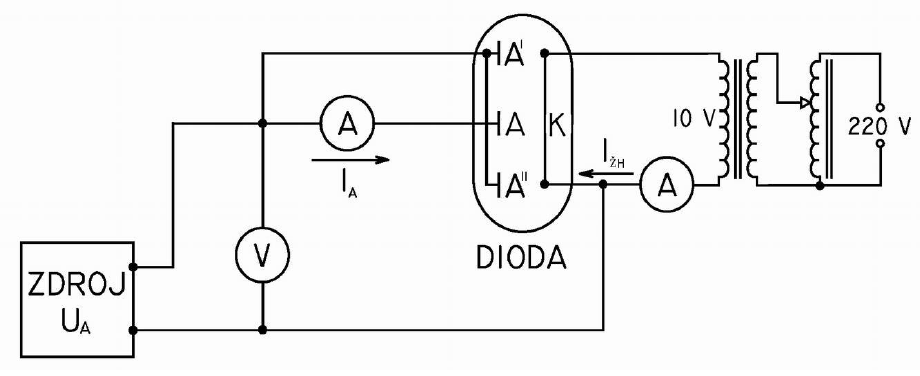
\includegraphics[width=12cm]{att/pyromet2.png}
%			\caption{Zapojení pro měření náběhového proudu. Převzato z \cite{bib:zadani}.}
%			\label{fig:s_aparatura_nasyc}
%			\end{figure}	
%			
%			\begin{figure}[h!]
%			\centering
%			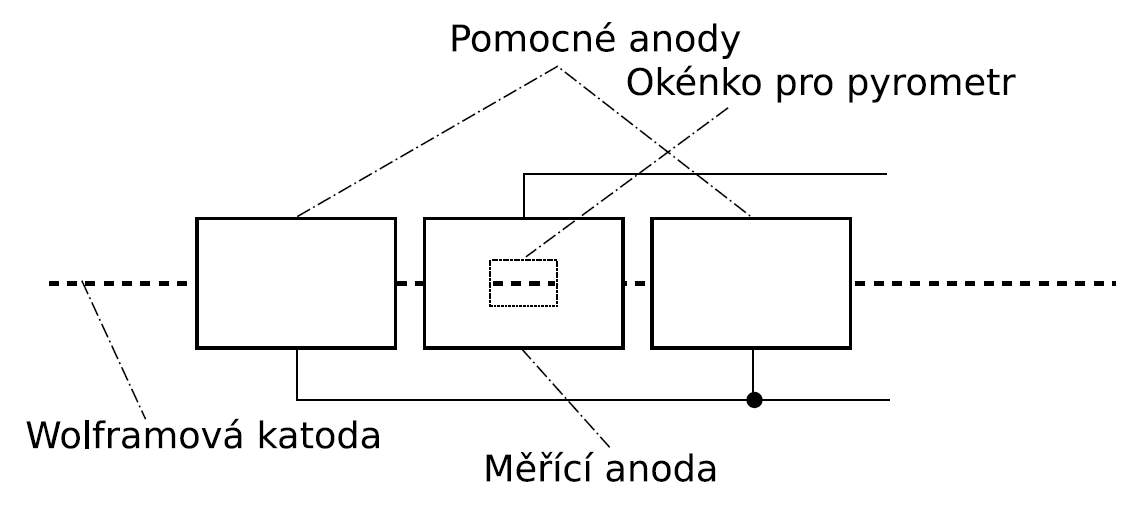
\includegraphics[width=10cm]{att/pyromet.png}
%			\caption{Geometrie uspořádání vakuové diody s pomocnými anodami pro dosažení homogenního pole. \newline Převzato z \cite{bib:zadani}.}
%			\label{fig:s_dida}
%			\end{figure}
%	
%\clearpage
\section{Tabulky a grafy}

%%
	\begin{figure}[h!]
	\begin{center}
	    \vspace*{-1cm}
		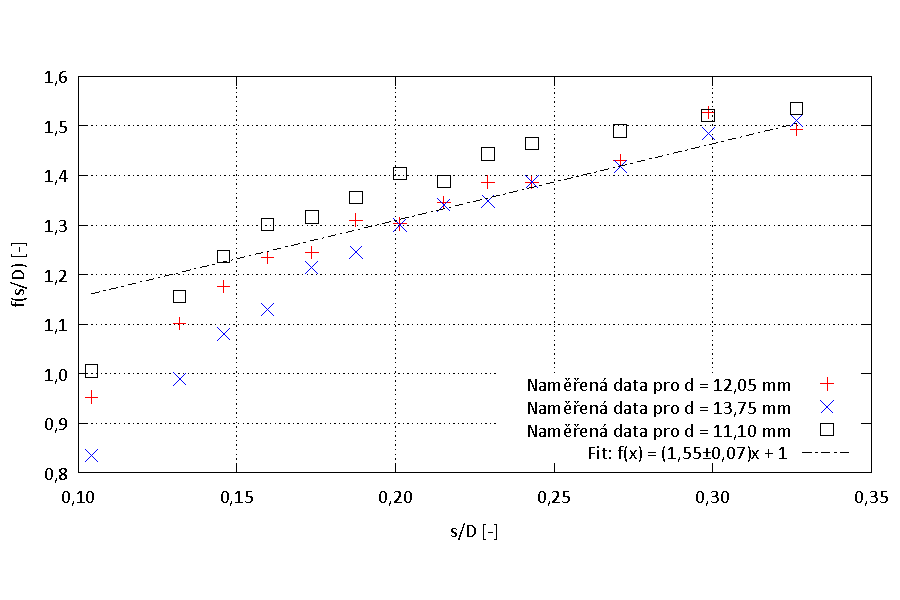
\includegraphics[width=\linewidth]{../gnuplot/pruraz.pdf}
	    \vspace*{-2cm}
		\caption{Naměřené hodnoty; závislost funkce $f(s/D)$ na poměru $s/D$. Hodnoty všech tří měření dohromady byly následně proloženy lineární závislostí $f(s/D) = a\cdot (s/D) + 1$.}
		\label{fig:g_pruraz}
	\end{center}
	\end{figure}
\clearpage

% Table generated by Excel2LaTeX from sheet 'List1'
\begin{table}[h!]
\catcode`\-=12 % HAX na enable cline v českym bable
  \centering
    \begin{tabular}{|r|r|r|}
    \hline
    \boldmath{}\textbf{$d$ [mm]}\unboldmath{} & \boldmath{}\textbf{$m$ [g]}\unboldmath{} & \boldmath{}\textbf{$E_p$ [MV/m]}\unboldmath{} \bigstrut\\
    \hline
    15,65 & 18,0  & 1,33 \bigstrut\\
    \hline
    12,85 & 15,5  & 1,23 \bigstrut\\
    \hline
    14,95 & 15,0  & 1,21 \bigstrut\\
    \hline
    11,40 & 19,0  & 1,36 \bigstrut\\
    \hline
    16,75 & 15,5  & 1,23 \bigstrut\\
    \hline
    7,20  & 20,5  & 1,41 \bigstrut\\
    \hline
    16,85 & 17,0  & 1,29 \bigstrut\\
    \hline
    13,05 & 18,0  & 1,33 \bigstrut\\
    \hline
    11,25 & 21,5  & 1,45 \bigstrut\\
    \hline
    9,30  & 23,0  & 1,50 \bigstrut\\
    \hline
    19,45 & 15,5  & 1,23 \bigstrut\\
    \hline
    10,45 & 23,0  & 1,50 \bigstrut\\
    \hline
    11,90 & 22,0  & 1,47 \bigstrut\\
    \hline
    \end{tabular}%
      \caption{
      		Naměřené a vypočítané hodnoty; měření dielektrické pevnosti vzduchu, $d$ je vzdálenost desek kondenzátoru s chybou 0,01~mm, $m$ hmotnost odečtená z vah s chybou 0,5~g a $E_p$ spočítaná dielektrická pevnost vzduchu podle vztahu (\ref{eq:Ep}). Chybu závěrečné hodnoty určíme z aritmetického průměru těchto hodnot.  
      }
      \label{tab:kondenzator}%
\end{table}%

% Table generated by Excel2LaTeX from sheet 'List1'
\begin{table}[h!]
\catcode`\-=12 % HAX na enable cline v českym bable
   \centering
    \begin{tabular}{|r|r|r|r|}
    \hline
    \boldmath{}\textbf{$s$ [mm]}\unboldmath{} & \boldmath{}\textbf{$m_1$ [g]}\unboldmath{} & \boldmath{}\textbf{$m_2$ [g]}\unboldmath{} & \boldmath{}\textbf{$m_3$ [g]}\unboldmath{} \bigstrut\\
    \hline
    1,5   & 3,5   & 3,5   & 3,7 \bigstrut\\
    \hline
    1,9   & 4,2   & 4,0   & 4,5 \bigstrut\\
    \hline
    2,1   & 4,5   & 4,1   & 4,8 \bigstrut\\
    \hline
    2,3   & 4,9   & 4,5   & 5,2 \bigstrut\\
    \hline
    2,5   & 5,7   & 4,6   & 6,0 \bigstrut\\
    \hline
    2,7   & 6,0   & 5,1   & 6,6 \bigstrut\\
    \hline
    2,9   & 7,0   & 5,4   & 7,1 \bigstrut\\
    \hline
    3,1   & 7,5   & 5,8   & 8,3 \bigstrut\\
    \hline
    3,3   & 8,0   & 6,5   & 8,7 \bigstrut\\
    \hline
    3,5   & 9,0   & 6,9   & 9,5 \bigstrut\\
    \hline
    3,9   & 10,5  & 8,2   & 11,4 \bigstrut\\
    \hline
    4,3   & 11,2  & 9,1   & 13,3 \bigstrut\\
    \hline
    4,7   & 14,0  & 10,5  & 15,6 \bigstrut\\
    \hline
    \end{tabular}%
       \caption{
            		Naměřené a vypočítané hodnoty; měření průrazu na kulovém jiskřišti, $s$ jsou na něm zvolené doskoky s chybou 0,1~mm a $m_{1-3}$ hmotnosti určené z vah s chybou $0,1$~g pro vzdálenosti desek kondenzátoru  $d_1=12,05$~mm, $d_2=13,75$~mm a $d_3=11,10$~mm s chybou $0,01$ mm.
            }
  \label{tab:jiskriste}%
\end{table}%


\clearpage	
	\begin{figure}[h!]
	\begin{center}
	    \vspace*{-1.5cm}
		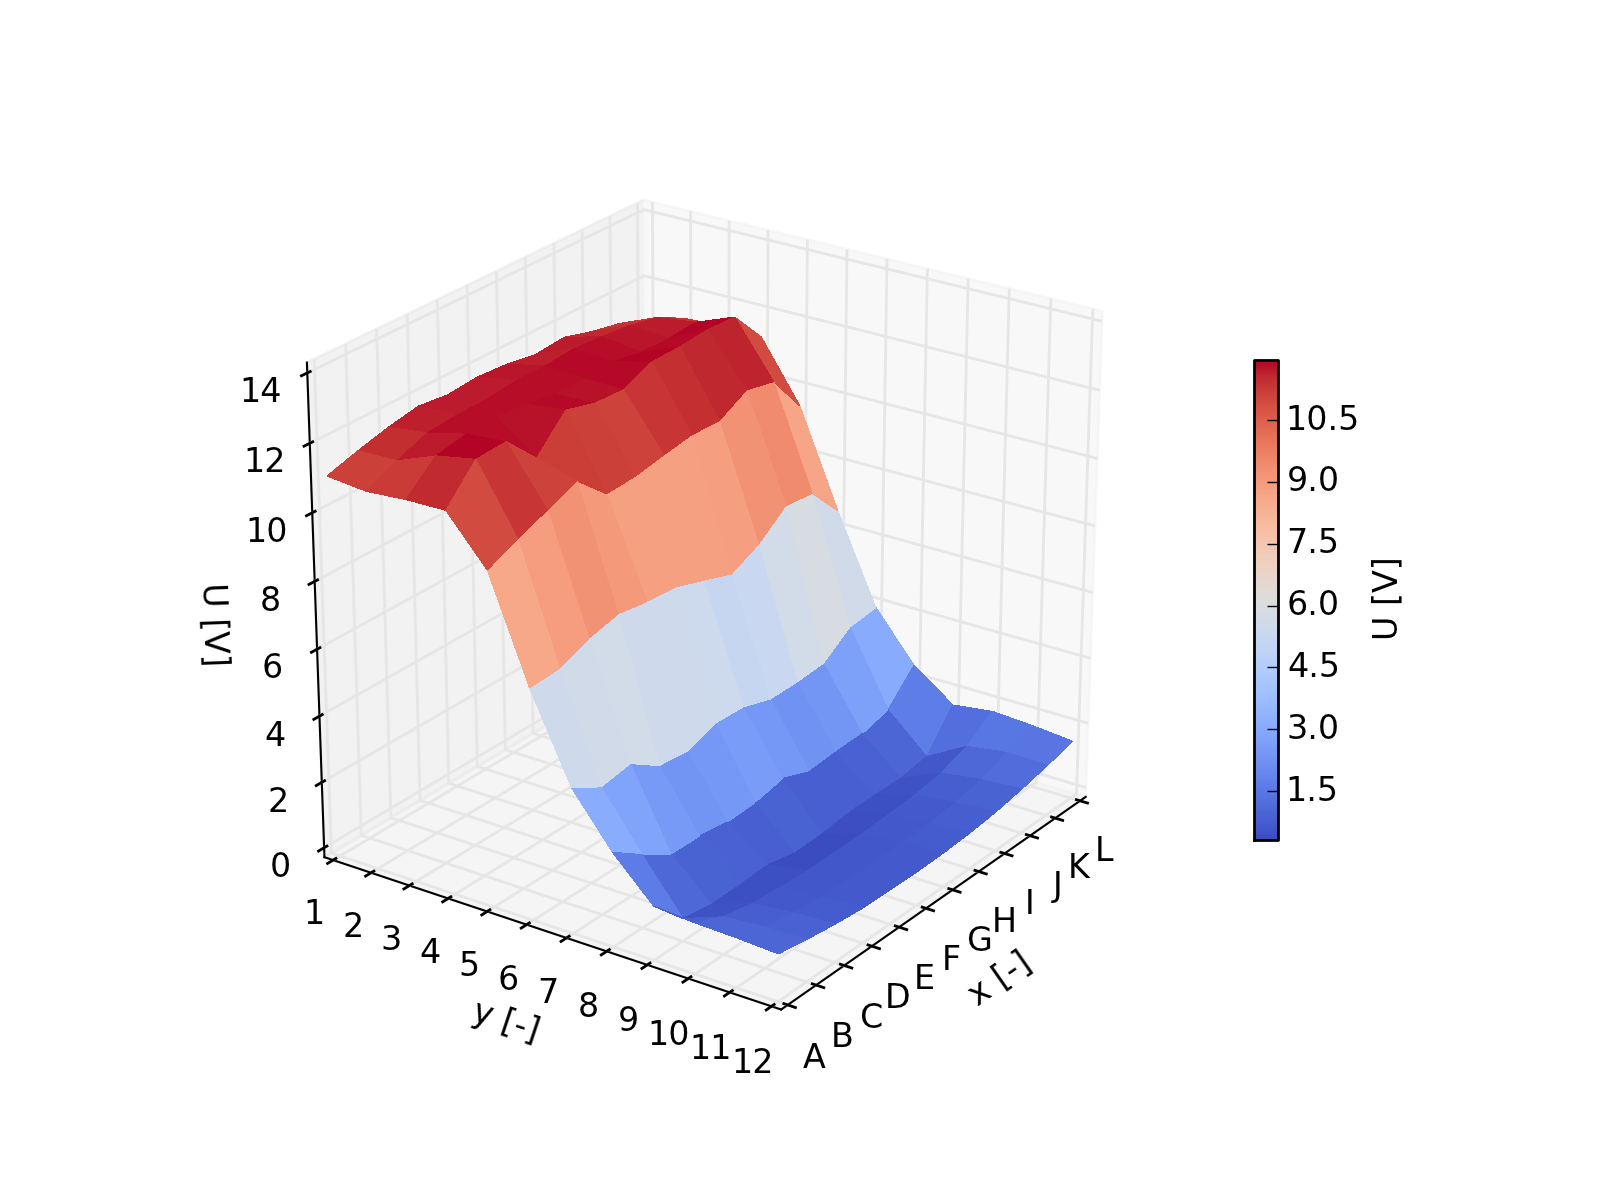
\includegraphics[width=\linewidth]{../gnuplot/konfigurace_1.png}
	    \vspace*{-2cm}
		\caption{Naměřené hodnoty; mapování potenciálu (napětí $U$) v závislosti na souřadnicích $x$ (A--L) a $y$ (1--12) při první konfiguraci elektrod.} 
		\label{fig:g_konf1}
	\end{center}
	\end{figure}			

	\begin{figure}[h!]
	\begin{center}
	    \vspace*{-0.5cm}
		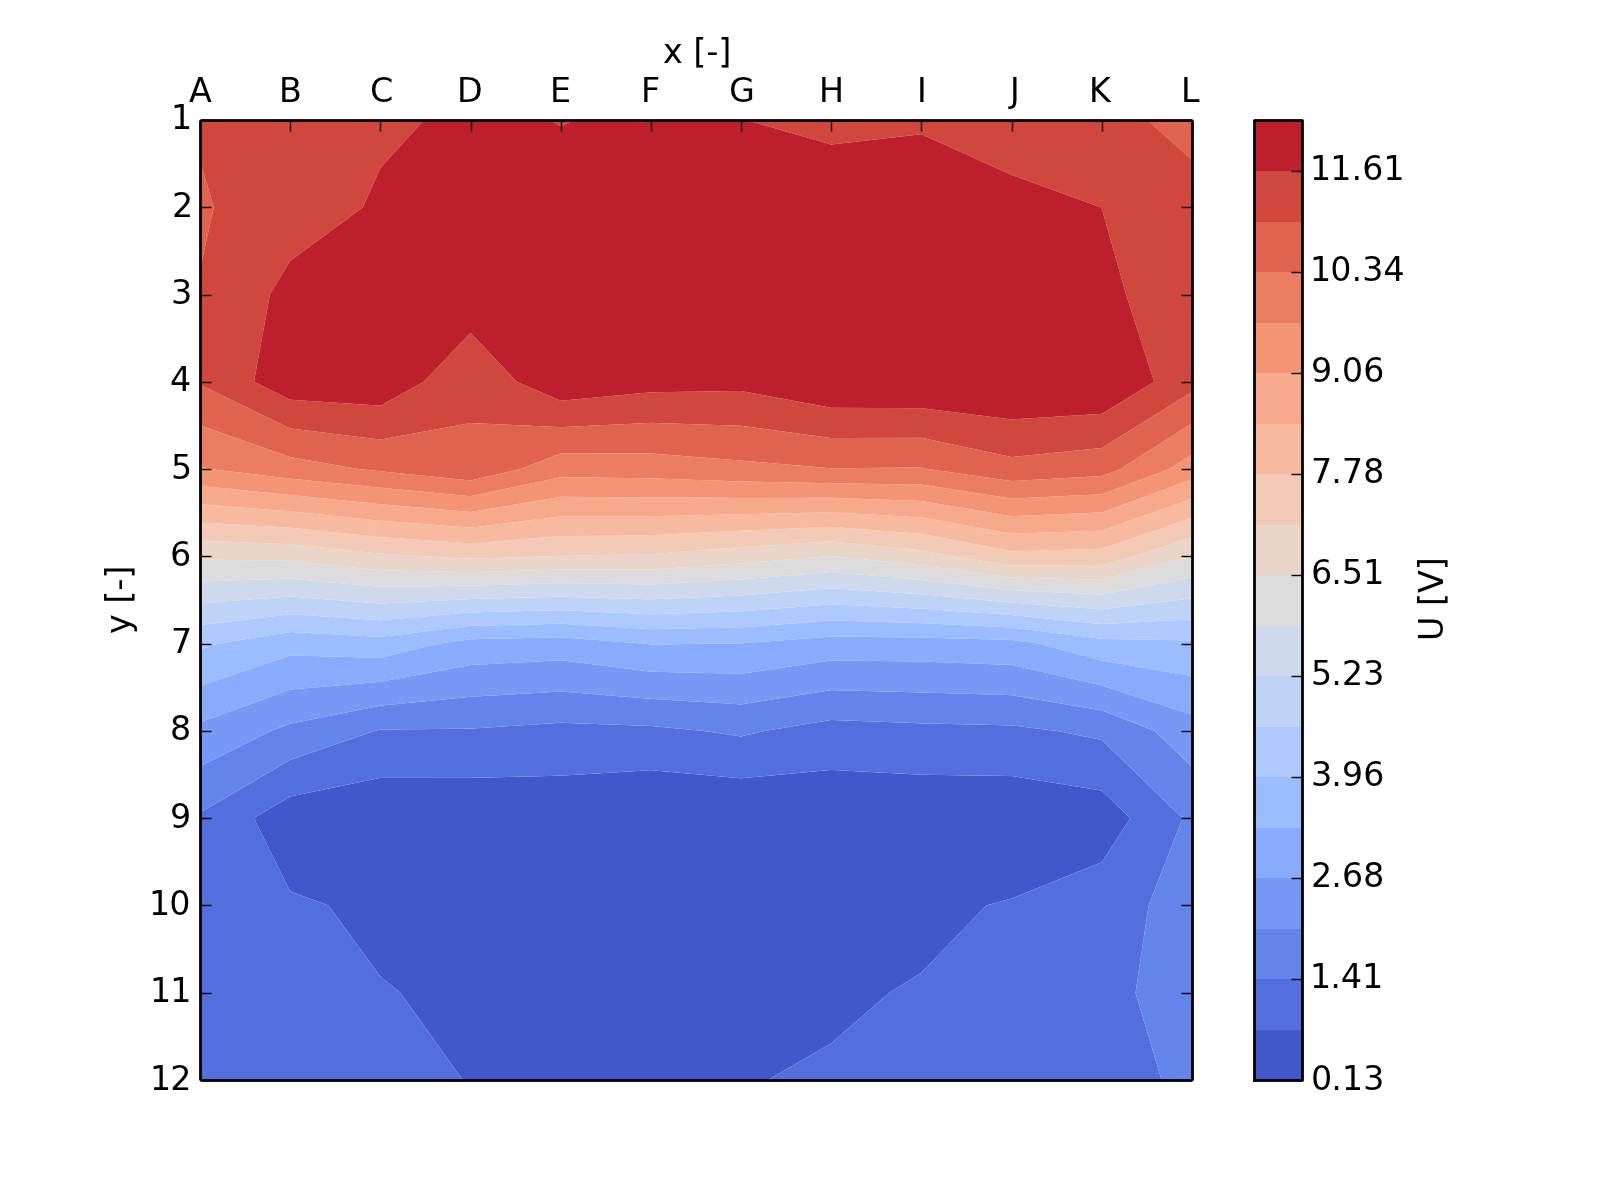
\includegraphics[width=0.8\linewidth]{../gnuplot/konfigurace_1_map.png}
	    \vspace*{-1cm}
		\caption{Naměřené hodnoty; mapování potenciálu (napětí $U$) při první konfiguraci elektrod na souřadnicích $x$ (A--L) a $y$ (1--12) (pohled shora).} 
		\label{fig:g_konf1_mapa}
	\end{center}
	\end{figure}
	\begin{figure}[h!]
	\begin{center}
	    \vspace*{-1.5cm}
		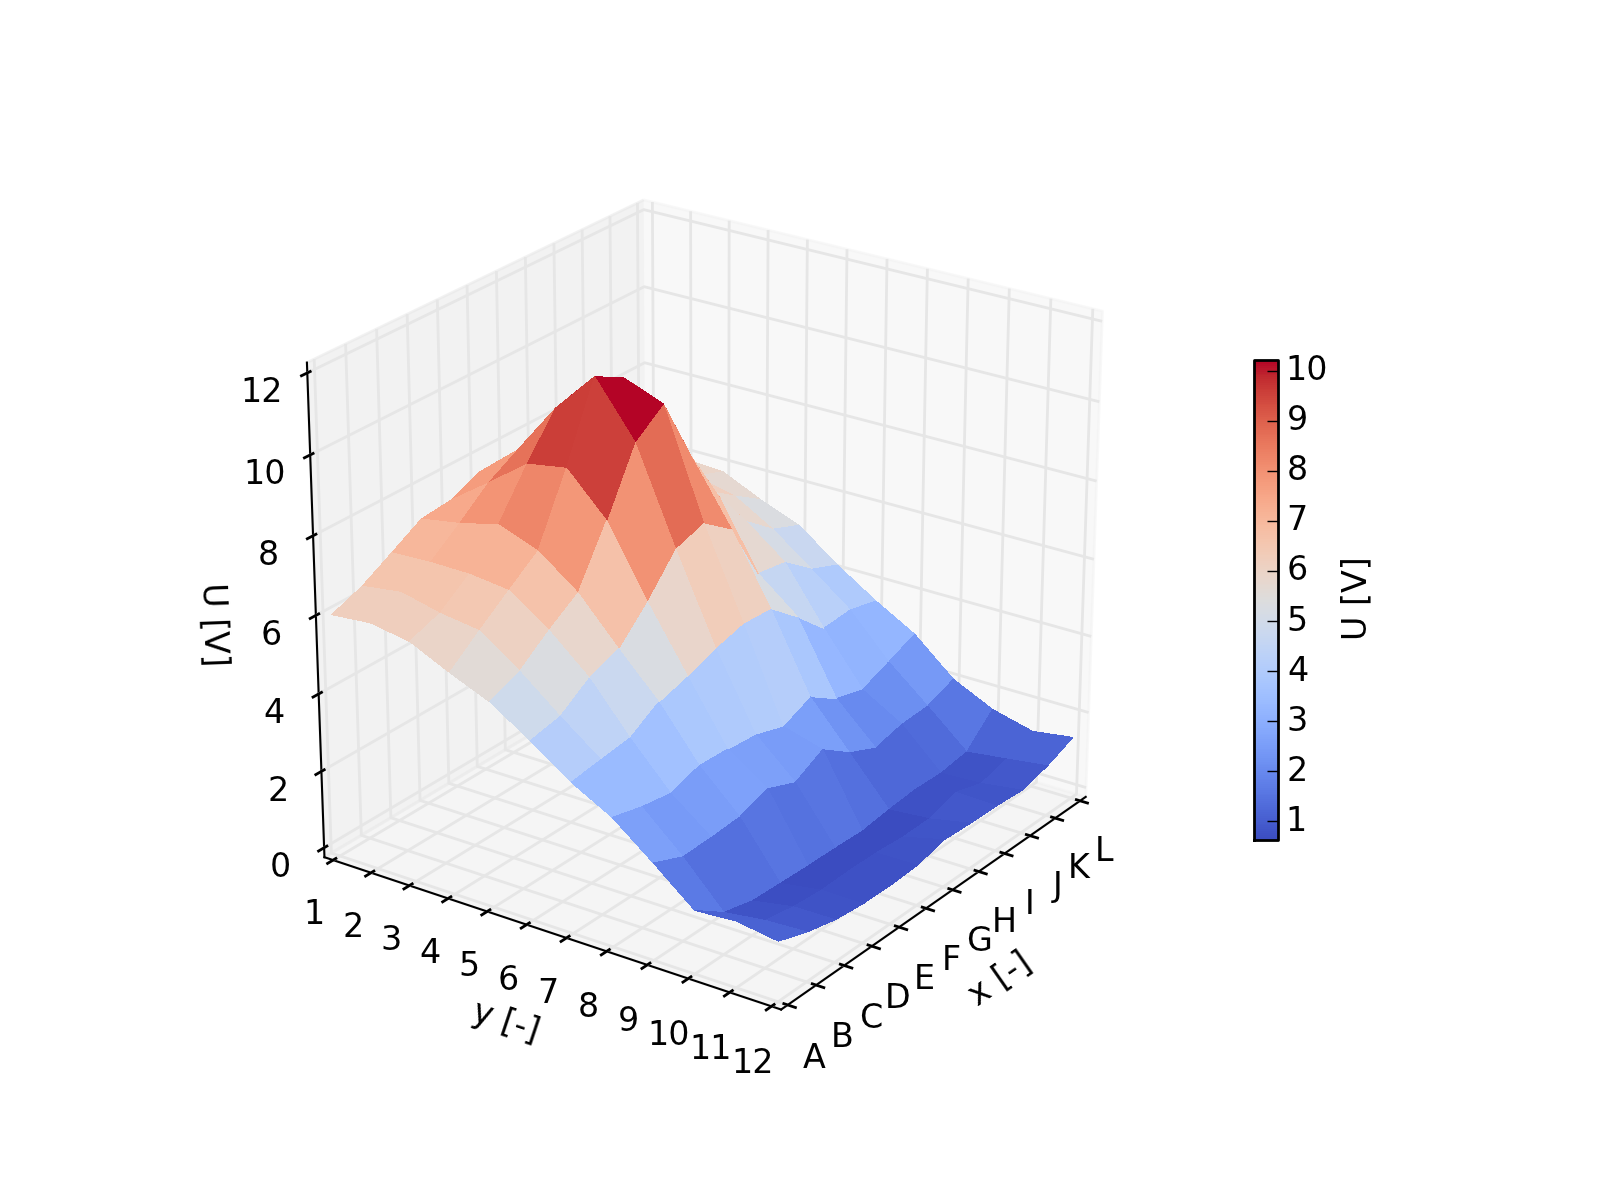
\includegraphics[width=\linewidth]{../gnuplot/konfigurace_2.png}
	    \vspace*{-2cm}
		\caption{Naměřené hodnoty; mapování potenciálu (napětí $U$) v závislosti na souřadnicích $x$ (A--L) a $y$ (1--12) při druhé konfiguraci elektrod.} 
		\label{fig:g_konf2}
	\end{center}
	\end{figure}			

	\begin{figure}[h!]
	\begin{center}
	    \vspace*{-0.5cm}
		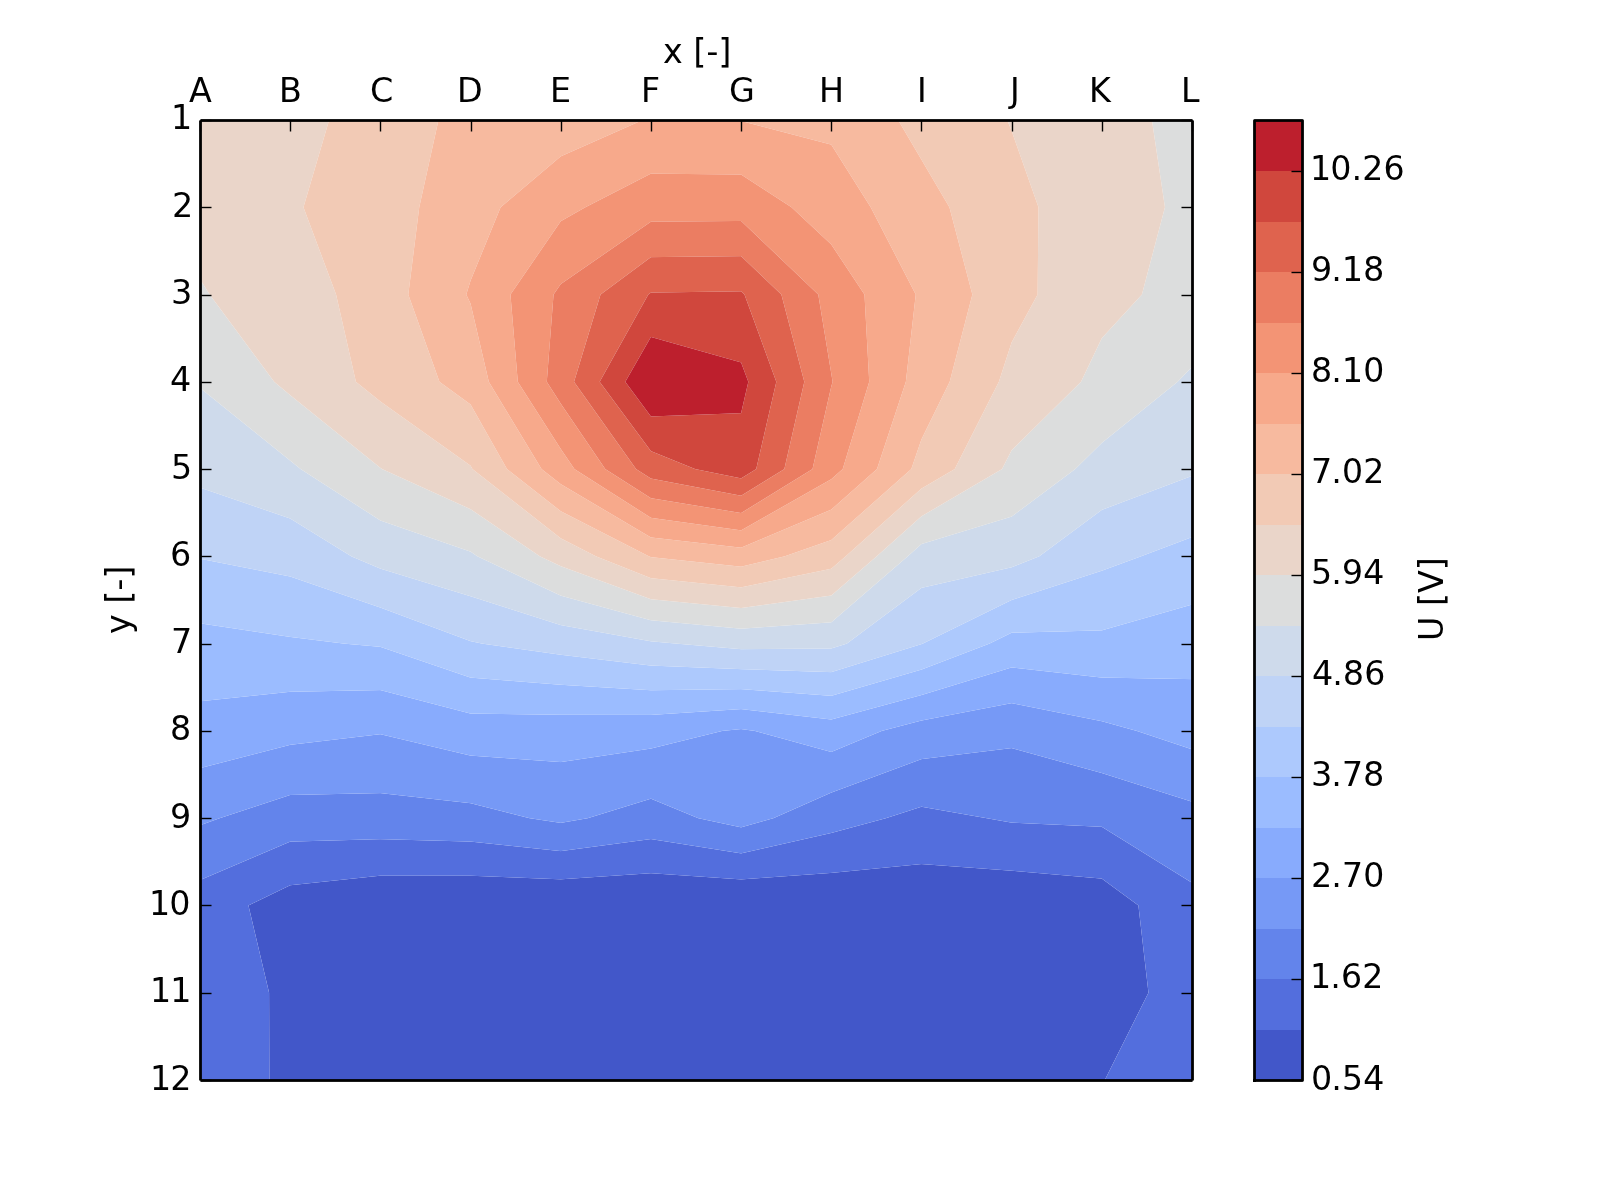
\includegraphics[width=0.8\linewidth]{../gnuplot/konfigurace_2_map.png}
	    \vspace*{-1cm}
		\caption{Naměřené hodnoty; mapování potenciálu (napětí $U$) při druhé konfiguraci elektrod na souřadnicích $x$ (A--L) a $y$ (1--12) (pohled shora).} 
		\label{fig:g_konf2_mapa}
	\end{center}
	\end{figure}

	\begin{figure}[h!]
	\begin{center}
	    \vspace*{-1.5cm}
		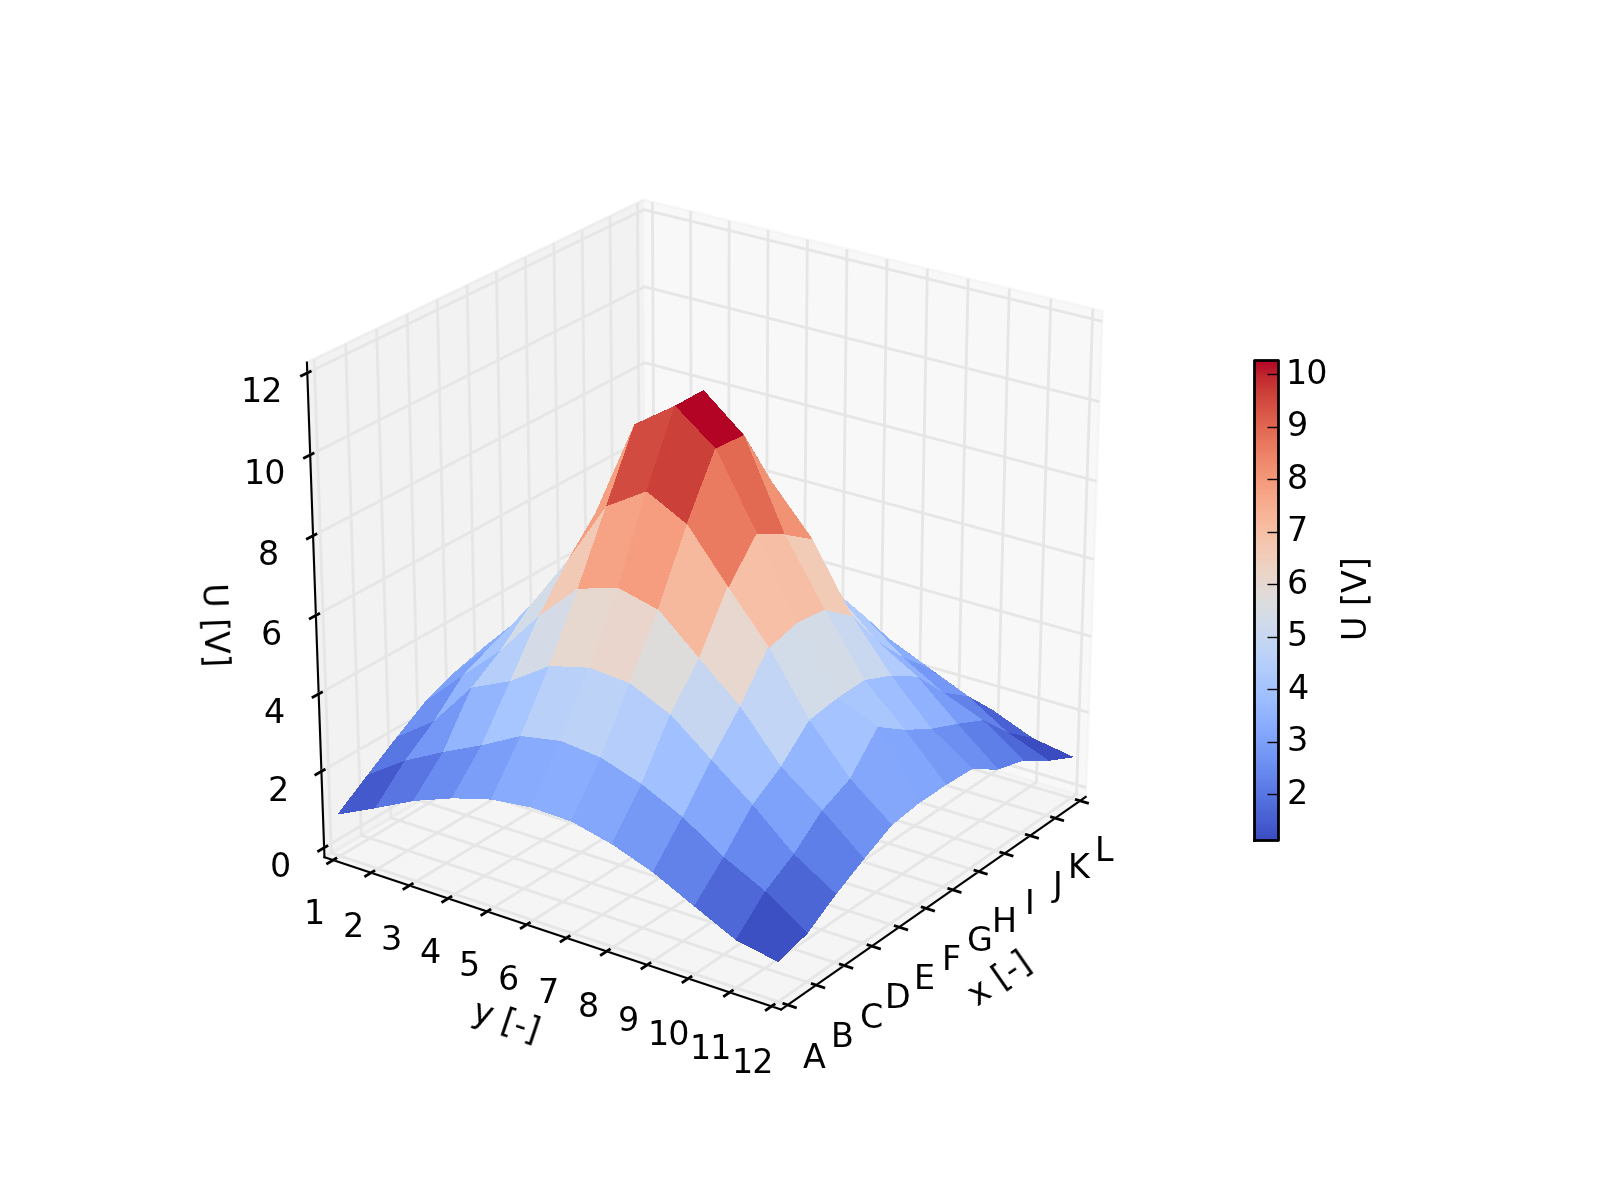
\includegraphics[width=\linewidth]{../gnuplot/konfigurace_3.png}
	    \vspace*{-2cm}
		\caption{Naměřené hodnoty; mapování potenciálu (napětí $U$) v závislosti na souřadnicích $x$ (A--L) a $y$ (1--12) při třetí konfiguraci elektrod.} 
		\label{fig:g_konf3}
	\end{center}
	\end{figure}			

	\begin{figure}[h!]
	\begin{center}
	    \vspace*{-0.5cm}
		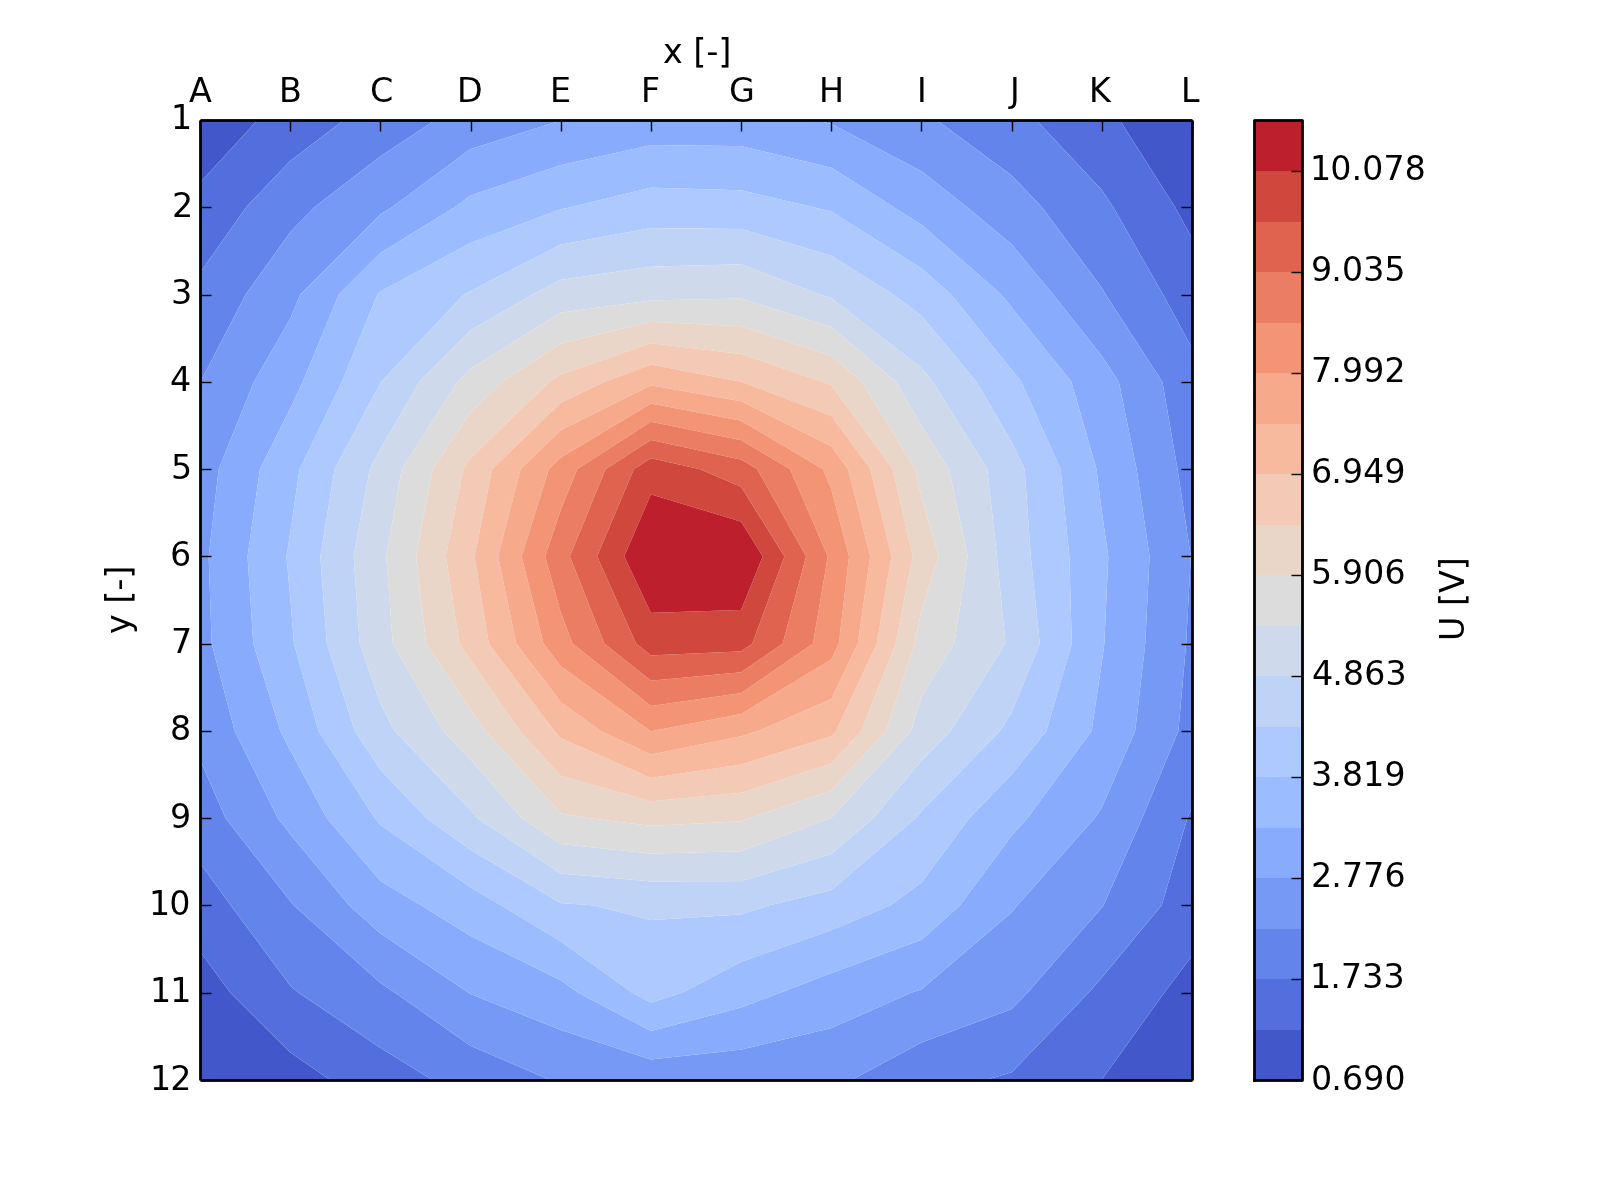
\includegraphics[width=0.8\linewidth]{../gnuplot/konfigurace_3_map.png}
	    \vspace*{-1cm}
		\caption{Naměřené hodnoty; mapování potenciálu (napětí $U$) při třetí konfiguraci elektrod na souřadnicích $x$ (A--L) a $y$ (1--12) (pohled shora).} 
		\label{fig:g_konf3_mapa}
	\end{center}
	\end{figure}
					
%\clearpage
% --- Konec dokumentu --------------------------------------------------


\end{document}

